% Options for packages loaded elsewhere
\PassOptionsToPackage{unicode}{hyperref}
\PassOptionsToPackage{hyphens}{url}
%
\documentclass[
]{article}
\usepackage{lmodern}
\usepackage{amssymb,amsmath}
\usepackage{ifxetex,ifluatex}
\ifnum 0\ifxetex 1\fi\ifluatex 1\fi=0 % if pdftex
  \usepackage[T1]{fontenc}
  \usepackage[utf8]{inputenc}
  \usepackage{textcomp} % provide euro and other symbols
\else % if luatex or xetex
  \usepackage{unicode-math}
  \defaultfontfeatures{Scale=MatchLowercase}
  \defaultfontfeatures[\rmfamily]{Ligatures=TeX,Scale=1}
\fi
% Use upquote if available, for straight quotes in verbatim environments
\IfFileExists{upquote.sty}{\usepackage{upquote}}{}
\IfFileExists{microtype.sty}{% use microtype if available
  \usepackage[]{microtype}
  \UseMicrotypeSet[protrusion]{basicmath} % disable protrusion for tt fonts
}{}
\makeatletter
\@ifundefined{KOMAClassName}{% if non-KOMA class
  \IfFileExists{parskip.sty}{%
    \usepackage{parskip}
  }{% else
    \setlength{\parindent}{0pt}
    \setlength{\parskip}{6pt plus 2pt minus 1pt}}
}{% if KOMA class
  \KOMAoptions{parskip=half}}
\makeatother
\usepackage{xcolor}
\IfFileExists{xurl.sty}{\usepackage{xurl}}{} % add URL line breaks if available
\IfFileExists{bookmark.sty}{\usepackage{bookmark}}{\usepackage{hyperref}}
\hypersetup{
  pdftitle={runif},
  pdfauthor={Joshua},
  hidelinks,
  pdfcreator={LaTeX via pandoc}}
\urlstyle{same} % disable monospaced font for URLs
\usepackage[margin=1in]{geometry}
\usepackage{color}
\usepackage{fancyvrb}
\newcommand{\VerbBar}{|}
\newcommand{\VERB}{\Verb[commandchars=\\\{\}]}
\DefineVerbatimEnvironment{Highlighting}{Verbatim}{commandchars=\\\{\}}
% Add ',fontsize=\small' for more characters per line
\usepackage{framed}
\definecolor{shadecolor}{RGB}{248,248,248}
\newenvironment{Shaded}{\begin{snugshade}}{\end{snugshade}}
\newcommand{\AlertTok}[1]{\textcolor[rgb]{0.94,0.16,0.16}{#1}}
\newcommand{\AnnotationTok}[1]{\textcolor[rgb]{0.56,0.35,0.01}{\textbf{\textit{#1}}}}
\newcommand{\AttributeTok}[1]{\textcolor[rgb]{0.77,0.63,0.00}{#1}}
\newcommand{\BaseNTok}[1]{\textcolor[rgb]{0.00,0.00,0.81}{#1}}
\newcommand{\BuiltInTok}[1]{#1}
\newcommand{\CharTok}[1]{\textcolor[rgb]{0.31,0.60,0.02}{#1}}
\newcommand{\CommentTok}[1]{\textcolor[rgb]{0.56,0.35,0.01}{\textit{#1}}}
\newcommand{\CommentVarTok}[1]{\textcolor[rgb]{0.56,0.35,0.01}{\textbf{\textit{#1}}}}
\newcommand{\ConstantTok}[1]{\textcolor[rgb]{0.00,0.00,0.00}{#1}}
\newcommand{\ControlFlowTok}[1]{\textcolor[rgb]{0.13,0.29,0.53}{\textbf{#1}}}
\newcommand{\DataTypeTok}[1]{\textcolor[rgb]{0.13,0.29,0.53}{#1}}
\newcommand{\DecValTok}[1]{\textcolor[rgb]{0.00,0.00,0.81}{#1}}
\newcommand{\DocumentationTok}[1]{\textcolor[rgb]{0.56,0.35,0.01}{\textbf{\textit{#1}}}}
\newcommand{\ErrorTok}[1]{\textcolor[rgb]{0.64,0.00,0.00}{\textbf{#1}}}
\newcommand{\ExtensionTok}[1]{#1}
\newcommand{\FloatTok}[1]{\textcolor[rgb]{0.00,0.00,0.81}{#1}}
\newcommand{\FunctionTok}[1]{\textcolor[rgb]{0.00,0.00,0.00}{#1}}
\newcommand{\ImportTok}[1]{#1}
\newcommand{\InformationTok}[1]{\textcolor[rgb]{0.56,0.35,0.01}{\textbf{\textit{#1}}}}
\newcommand{\KeywordTok}[1]{\textcolor[rgb]{0.13,0.29,0.53}{\textbf{#1}}}
\newcommand{\NormalTok}[1]{#1}
\newcommand{\OperatorTok}[1]{\textcolor[rgb]{0.81,0.36,0.00}{\textbf{#1}}}
\newcommand{\OtherTok}[1]{\textcolor[rgb]{0.56,0.35,0.01}{#1}}
\newcommand{\PreprocessorTok}[1]{\textcolor[rgb]{0.56,0.35,0.01}{\textit{#1}}}
\newcommand{\RegionMarkerTok}[1]{#1}
\newcommand{\SpecialCharTok}[1]{\textcolor[rgb]{0.00,0.00,0.00}{#1}}
\newcommand{\SpecialStringTok}[1]{\textcolor[rgb]{0.31,0.60,0.02}{#1}}
\newcommand{\StringTok}[1]{\textcolor[rgb]{0.31,0.60,0.02}{#1}}
\newcommand{\VariableTok}[1]{\textcolor[rgb]{0.00,0.00,0.00}{#1}}
\newcommand{\VerbatimStringTok}[1]{\textcolor[rgb]{0.31,0.60,0.02}{#1}}
\newcommand{\WarningTok}[1]{\textcolor[rgb]{0.56,0.35,0.01}{\textbf{\textit{#1}}}}
\usepackage{graphicx,grffile}
\makeatletter
\def\maxwidth{\ifdim\Gin@nat@width>\linewidth\linewidth\else\Gin@nat@width\fi}
\def\maxheight{\ifdim\Gin@nat@height>\textheight\textheight\else\Gin@nat@height\fi}
\makeatother
% Scale images if necessary, so that they will not overflow the page
% margins by default, and it is still possible to overwrite the defaults
% using explicit options in \includegraphics[width, height, ...]{}
\setkeys{Gin}{width=\maxwidth,height=\maxheight,keepaspectratio}
% Set default figure placement to htbp
\makeatletter
\def\fps@figure{htbp}
\makeatother
\setlength{\emergencystretch}{3em} % prevent overfull lines
\providecommand{\tightlist}{%
  \setlength{\itemsep}{0pt}\setlength{\parskip}{0pt}}
\setcounter{secnumdepth}{-\maxdimen} % remove section numbering

\title{runif}
\author{Joshua}
\date{25/05/2020}

\begin{document}
\maketitle

\begin{Shaded}
\begin{Highlighting}[]
\NormalTok{knitr}\OperatorTok{::}\NormalTok{opts_chunk}\OperatorTok{$}\KeywordTok{set}\NormalTok{(}\DataTypeTok{echo =} \OtherTok{TRUE}\NormalTok{)}
\KeywordTok{rm}\NormalTok{(}\DataTypeTok{list=}\KeywordTok{ls}\NormalTok{())}
\KeywordTok{library}\NormalTok{(}\StringTok{'forecast'}\NormalTok{)}
\end{Highlighting}
\end{Shaded}

\begin{verbatim}
## Warning: package 'forecast' was built under R version 3.5.2
\end{verbatim}

\begin{Shaded}
\begin{Highlighting}[]
\KeywordTok{library}\NormalTok{(}\StringTok{'smooth'}\NormalTok{)}
\end{Highlighting}
\end{Shaded}

\begin{verbatim}
## Warning: package 'smooth' was built under R version 3.5.2
\end{verbatim}

\begin{verbatim}
## Loading required package: greybox
\end{verbatim}

\begin{verbatim}
## Warning: package 'greybox' was built under R version 3.5.2
\end{verbatim}

\begin{verbatim}
## Package "greybox", v0.5.8 loaded.
\end{verbatim}

\begin{verbatim}
## This is package "smooth", v2.5.5
\end{verbatim}

\begin{Shaded}
\begin{Highlighting}[]
\KeywordTok{library}\NormalTok{(}\StringTok{'beanplot'}\NormalTok{)}
\KeywordTok{library}\NormalTok{(}\StringTok{'pastecs'}\NormalTok{)}
\KeywordTok{library}\NormalTok{(}\StringTok{'scales'}\NormalTok{)}
\KeywordTok{library}\NormalTok{(}\StringTok{'ggplot2'}\NormalTok{)}

\KeywordTok{load}\NormalTok{(}\StringTok{'runif.Rdata'}\NormalTok{)}


\NormalTok{iter<-}\DecValTok{20000}
\end{Highlighting}
\end{Shaded}

\hypertarget{ppl-vs-length}{%
\subsection{ppl vs length}\label{ppl-vs-length}}

\begin{Shaded}
\begin{Highlighting}[]
\NormalTok{x_axis<-}\KeywordTok{c}\NormalTok{(}\DecValTok{40}\NormalTok{,}\DecValTok{120}\NormalTok{,}\DecValTok{480}\NormalTok{,}\DecValTok{1200}\NormalTok{,}\DecValTok{4800}\NormalTok{)}
\NormalTok{y_}\DecValTok{40}\NormalTok{<-}\KeywordTok{c}\NormalTok{(}\KeywordTok{mean}\NormalTok{(}\KeywordTok{sapply}\NormalTok{(re_}\DecValTok{40}\NormalTok{[[}\DecValTok{1}\NormalTok{]], }\StringTok{"[["}\NormalTok{, }\DecValTok{1}\NormalTok{)),}\KeywordTok{mean}\NormalTok{(}\KeywordTok{sapply}\NormalTok{(re_}\DecValTok{40}\NormalTok{[[}\DecValTok{2}\NormalTok{]], }\StringTok{"[["}\NormalTok{, }\DecValTok{1}\NormalTok{)),}
        \KeywordTok{mean}\NormalTok{(}\KeywordTok{sapply}\NormalTok{(re_}\DecValTok{40}\NormalTok{[[}\DecValTok{3}\NormalTok{]], }\StringTok{"[["}\NormalTok{, }\DecValTok{1}\NormalTok{)))}
\NormalTok{y_}\DecValTok{120}\NormalTok{<-}\KeywordTok{c}\NormalTok{(}\KeywordTok{mean}\NormalTok{(}\KeywordTok{sapply}\NormalTok{(re_}\DecValTok{120}\NormalTok{[[}\DecValTok{1}\NormalTok{]], }\StringTok{"[["}\NormalTok{, }\DecValTok{1}\NormalTok{)),}\KeywordTok{mean}\NormalTok{(}\KeywordTok{sapply}\NormalTok{(re_}\DecValTok{120}\NormalTok{[[}\DecValTok{2}\NormalTok{]], }\StringTok{"[["}\NormalTok{, }\DecValTok{1}\NormalTok{)),}
        \KeywordTok{mean}\NormalTok{(}\KeywordTok{sapply}\NormalTok{(re_}\DecValTok{120}\NormalTok{[[}\DecValTok{3}\NormalTok{]], }\StringTok{"[["}\NormalTok{, }\DecValTok{1}\NormalTok{)))}
\NormalTok{y_}\DecValTok{480}\NormalTok{<-}\KeywordTok{c}\NormalTok{(}\KeywordTok{mean}\NormalTok{(}\KeywordTok{sapply}\NormalTok{(re_}\DecValTok{480}\NormalTok{[[}\DecValTok{1}\NormalTok{]], }\StringTok{"[["}\NormalTok{, }\DecValTok{1}\NormalTok{)),}\KeywordTok{mean}\NormalTok{(}\KeywordTok{sapply}\NormalTok{(re_}\DecValTok{480}\NormalTok{[[}\DecValTok{2}\NormalTok{]], }\StringTok{"[["}\NormalTok{, }\DecValTok{1}\NormalTok{)),}
        \KeywordTok{mean}\NormalTok{(}\KeywordTok{sapply}\NormalTok{(re_}\DecValTok{480}\NormalTok{[[}\DecValTok{3}\NormalTok{]], }\StringTok{"[["}\NormalTok{, }\DecValTok{1}\NormalTok{)))}
\NormalTok{y_}\DecValTok{1200}\NormalTok{<-}\KeywordTok{c}\NormalTok{(}\KeywordTok{mean}\NormalTok{(}\KeywordTok{sapply}\NormalTok{(re_}\DecValTok{1200}\NormalTok{[[}\DecValTok{1}\NormalTok{]], }\StringTok{"[["}\NormalTok{, }\DecValTok{1}\NormalTok{)),}\KeywordTok{mean}\NormalTok{(}\KeywordTok{sapply}\NormalTok{(re_}\DecValTok{1200}\NormalTok{[[}\DecValTok{2}\NormalTok{]], }\StringTok{"[["}\NormalTok{, }\DecValTok{1}\NormalTok{)),}
        \KeywordTok{mean}\NormalTok{(}\KeywordTok{sapply}\NormalTok{(re_}\DecValTok{1200}\NormalTok{[[}\DecValTok{3}\NormalTok{]], }\StringTok{"[["}\NormalTok{, }\DecValTok{1}\NormalTok{)))}
\NormalTok{y_}\DecValTok{4800}\NormalTok{<-}\KeywordTok{c}\NormalTok{(}\KeywordTok{mean}\NormalTok{(}\KeywordTok{sapply}\NormalTok{(re_}\DecValTok{4800}\NormalTok{[[}\DecValTok{1}\NormalTok{]], }\StringTok{"[["}\NormalTok{, }\DecValTok{1}\NormalTok{)),}\KeywordTok{mean}\NormalTok{(}\KeywordTok{sapply}\NormalTok{(re_}\DecValTok{4800}\NormalTok{[[}\DecValTok{2}\NormalTok{]], }\StringTok{"[["}\NormalTok{, }\DecValTok{1}\NormalTok{)),}
        \KeywordTok{mean}\NormalTok{(}\KeywordTok{sapply}\NormalTok{(re_}\DecValTok{4800}\NormalTok{[[}\DecValTok{3}\NormalTok{]], }\StringTok{"[["}\NormalTok{, }\DecValTok{1}\NormalTok{)))}
\NormalTok{y_axis<-}\KeywordTok{c}\NormalTok{(y_}\DecValTok{40}\NormalTok{,y_}\DecValTok{120}\NormalTok{,y_}\DecValTok{480}\NormalTok{,y_}\DecValTok{1200}\NormalTok{,y_}\DecValTok{4800}\NormalTok{)}
\NormalTok{mac<-}\KeywordTok{matrix}\NormalTok{(y_axis,}\DataTypeTok{nrow =} \DecValTok{3}\NormalTok{,}\DataTypeTok{ncol =} \DecValTok{5}\NormalTok{)}
\NormalTok{mac<-}\KeywordTok{t}\NormalTok{(mac)}
\KeywordTok{rownames}\NormalTok{(mac)<-}\KeywordTok{c}\NormalTok{(}\StringTok{'40'}\NormalTok{,}\StringTok{'120'}\NormalTok{,}\StringTok{'480'}\NormalTok{,}\StringTok{'1200'}\NormalTok{,}\StringTok{'4800'}\NormalTok{)}
\KeywordTok{colnames}\NormalTok{(mac)<-}\KeywordTok{c}\NormalTok{(}\StringTok{"DGP"}\NormalTok{, }\StringTok{"DJ"}\NormalTok{,}\StringTok{"CF"}\NormalTok{)}
\NormalTok{mac}
\end{Highlighting}
\end{Shaded}

\begin{verbatim}
##             DGP         DJ         CF
## 40   0.05236999 0.05729761 0.05914920
## 120  0.05067413 0.05383036 0.05367412
## 480  0.05030789 0.05161920 0.05175162
## 1200 0.05086648 0.05145084 0.05202975
## 4800 0.05164572 0.05127352 0.05270124
\end{verbatim}

\begin{Shaded}
\begin{Highlighting}[]
\NormalTok{v_}\DecValTok{40}\NormalTok{<-}\KeywordTok{c}\NormalTok{(}\KeywordTok{sd}\NormalTok{(}\KeywordTok{sapply}\NormalTok{(re_}\DecValTok{40}\NormalTok{[[}\DecValTok{1}\NormalTok{]], }\StringTok{"[["}\NormalTok{, }\DecValTok{1}\NormalTok{)),}\KeywordTok{sd}\NormalTok{(}\KeywordTok{sapply}\NormalTok{(re_}\DecValTok{40}\NormalTok{[[}\DecValTok{2}\NormalTok{]], }\StringTok{"[["}\NormalTok{, }\DecValTok{1}\NormalTok{)),}
        \KeywordTok{sd}\NormalTok{(}\KeywordTok{sapply}\NormalTok{(re_}\DecValTok{40}\NormalTok{[[}\DecValTok{3}\NormalTok{]], }\StringTok{"[["}\NormalTok{, }\DecValTok{1}\NormalTok{)))}
\NormalTok{v_}\DecValTok{120}\NormalTok{<-}\KeywordTok{c}\NormalTok{(}\KeywordTok{sd}\NormalTok{(}\KeywordTok{sapply}\NormalTok{(re_}\DecValTok{120}\NormalTok{[[}\DecValTok{1}\NormalTok{]], }\StringTok{"[["}\NormalTok{, }\DecValTok{1}\NormalTok{)),}\KeywordTok{sd}\NormalTok{(}\KeywordTok{sapply}\NormalTok{(re_}\DecValTok{120}\NormalTok{[[}\DecValTok{2}\NormalTok{]], }\StringTok{"[["}\NormalTok{, }\DecValTok{1}\NormalTok{)),}
        \KeywordTok{sd}\NormalTok{(}\KeywordTok{sapply}\NormalTok{(re_}\DecValTok{120}\NormalTok{[[}\DecValTok{3}\NormalTok{]], }\StringTok{"[["}\NormalTok{, }\DecValTok{1}\NormalTok{)))}
\NormalTok{v_}\DecValTok{480}\NormalTok{<-}\KeywordTok{c}\NormalTok{(}\KeywordTok{sd}\NormalTok{(}\KeywordTok{sapply}\NormalTok{(re_}\DecValTok{480}\NormalTok{[[}\DecValTok{1}\NormalTok{]], }\StringTok{"[["}\NormalTok{, }\DecValTok{1}\NormalTok{)),}\KeywordTok{sd}\NormalTok{(}\KeywordTok{sapply}\NormalTok{(re_}\DecValTok{480}\NormalTok{[[}\DecValTok{2}\NormalTok{]], }\StringTok{"[["}\NormalTok{, }\DecValTok{1}\NormalTok{)),}
        \KeywordTok{sd}\NormalTok{(}\KeywordTok{sapply}\NormalTok{(re_}\DecValTok{480}\NormalTok{[[}\DecValTok{3}\NormalTok{]], }\StringTok{"[["}\NormalTok{, }\DecValTok{1}\NormalTok{)))}
\NormalTok{v_}\DecValTok{1200}\NormalTok{<-}\KeywordTok{c}\NormalTok{(}\KeywordTok{sd}\NormalTok{(}\KeywordTok{sapply}\NormalTok{(re_}\DecValTok{1200}\NormalTok{[[}\DecValTok{1}\NormalTok{]], }\StringTok{"[["}\NormalTok{, }\DecValTok{1}\NormalTok{)),}\KeywordTok{sd}\NormalTok{(}\KeywordTok{sapply}\NormalTok{(re_}\DecValTok{1200}\NormalTok{[[}\DecValTok{2}\NormalTok{]], }\StringTok{"[["}\NormalTok{, }\DecValTok{1}\NormalTok{)),}
        \KeywordTok{sd}\NormalTok{(}\KeywordTok{sapply}\NormalTok{(re_}\DecValTok{1200}\NormalTok{[[}\DecValTok{3}\NormalTok{]], }\StringTok{"[["}\NormalTok{, }\DecValTok{1}\NormalTok{)))}
\NormalTok{v_}\DecValTok{4800}\NormalTok{<-}\KeywordTok{c}\NormalTok{(}\KeywordTok{sd}\NormalTok{(}\KeywordTok{sapply}\NormalTok{(re_}\DecValTok{4800}\NormalTok{[[}\DecValTok{1}\NormalTok{]], }\StringTok{"[["}\NormalTok{, }\DecValTok{1}\NormalTok{)),}\KeywordTok{sd}\NormalTok{(}\KeywordTok{sapply}\NormalTok{(re_}\DecValTok{4800}\NormalTok{[[}\DecValTok{2}\NormalTok{]], }\StringTok{"[["}\NormalTok{, }\DecValTok{1}\NormalTok{)),}
        \KeywordTok{sd}\NormalTok{(}\KeywordTok{sapply}\NormalTok{(re_}\DecValTok{4800}\NormalTok{[[}\DecValTok{3}\NormalTok{]], }\StringTok{"[["}\NormalTok{, }\DecValTok{1}\NormalTok{)))}
\NormalTok{v_axis<-}\KeywordTok{c}\NormalTok{(v_}\DecValTok{40}\NormalTok{,v_}\DecValTok{120}\NormalTok{,v_}\DecValTok{480}\NormalTok{,v_}\DecValTok{1200}\NormalTok{,v_}\DecValTok{4800}\NormalTok{)}
\NormalTok{var<-}\KeywordTok{matrix}\NormalTok{(v_axis,}\DataTypeTok{nrow =} \DecValTok{3}\NormalTok{,}\DataTypeTok{ncol =} \DecValTok{5}\NormalTok{)}
\NormalTok{var<-}\KeywordTok{t}\NormalTok{(var)}
\KeywordTok{rownames}\NormalTok{(var)<-}\KeywordTok{c}\NormalTok{(}\StringTok{'40'}\NormalTok{,}\StringTok{'120'}\NormalTok{,}\StringTok{'480'}\NormalTok{,}\StringTok{'1200'}\NormalTok{,}\StringTok{'4800'}\NormalTok{)}
\KeywordTok{colnames}\NormalTok{(var)<-}\KeywordTok{c}\NormalTok{(}\StringTok{"DGP"}\NormalTok{, }\StringTok{"DJ"}\NormalTok{,}\StringTok{"CF"}\NormalTok{)}
\NormalTok{var}
\end{Highlighting}
\end{Shaded}

\begin{verbatim}
##             DGP         DJ         CF
## 40   0.09527237 0.09396095 0.11385300
## 120  0.08822607 0.08375629 0.09396513
## 480  0.14236613 0.13027228 0.14738238
## 1200 0.09314779 0.08680173 0.09523008
## 4800 0.10753826 0.10128942 0.10805198
\end{verbatim}

\begin{Shaded}
\begin{Highlighting}[]
\KeywordTok{par}\NormalTok{(}\DataTypeTok{mar=}\KeywordTok{c}\NormalTok{(}\KeywordTok{par}\NormalTok{(}\StringTok{'mar'}\NormalTok{)[}\DecValTok{1}\OperatorTok{:}\DecValTok{3}\NormalTok{], }\DecValTok{0}\NormalTok{)) }
\KeywordTok{plot.new}\NormalTok{()}
\NormalTok{l <-}\StringTok{ }\KeywordTok{legend}\NormalTok{(}\DecValTok{0}\NormalTok{, }\DecValTok{0}\NormalTok{, }\DataTypeTok{bty=}\StringTok{'n'}\NormalTok{,}\KeywordTok{c}\NormalTok{(}\StringTok{"DGP"}\NormalTok{, }\StringTok{"DJ"}\NormalTok{,}\StringTok{"PM"}\NormalTok{),}\DataTypeTok{plot=}\OtherTok{FALSE}\NormalTok{, }\DataTypeTok{pch=}\DecValTok{1}\OperatorTok{:}\DecValTok{3}\NormalTok{,}\DataTypeTok{col=}\DecValTok{1}\OperatorTok{:}\DecValTok{3}\NormalTok{)}
\NormalTok{w <-}\StringTok{ }\KeywordTok{grconvertX}\NormalTok{(l}\OperatorTok{$}\NormalTok{rect}\OperatorTok{$}\NormalTok{w, }\DataTypeTok{to=}\StringTok{'ndc'}\NormalTok{) }\OperatorTok{-}\StringTok{ }\KeywordTok{grconvertX}\NormalTok{(}\DecValTok{0}\NormalTok{, }\DataTypeTok{to=}\StringTok{'ndc'}\NormalTok{)}
\KeywordTok{par}\NormalTok{(}\DataTypeTok{omd=}\KeywordTok{c}\NormalTok{(}\DecValTok{0}\NormalTok{, }\DecValTok{1}\OperatorTok{-}\NormalTok{w, }\DecValTok{0}\NormalTok{, }\DecValTok{1}\NormalTok{))}
\KeywordTok{matplot}\NormalTok{(mac, }\DataTypeTok{type =} \KeywordTok{c}\NormalTok{(}\StringTok{"b"}\NormalTok{),}\DataTypeTok{pch=}\DecValTok{1}\OperatorTok{:}\DecValTok{3}\NormalTok{,}\DataTypeTok{col =} \DecValTok{1}\OperatorTok{:}\DecValTok{3}\NormalTok{,}\DataTypeTok{xaxt =} \StringTok{"n"}\NormalTok{,}\DataTypeTok{yaxt =} \StringTok{"n"}
\NormalTok{        ,}\DataTypeTok{xlab =} \StringTok{'data length'}\NormalTok{,}\DataTypeTok{ylab =} \StringTok{'percetage profit loss'}\NormalTok{) }
\KeywordTok{axis}\NormalTok{(}\DecValTok{1}\NormalTok{, }\DataTypeTok{at=}\DecValTok{1}\OperatorTok{:}\DecValTok{5}\NormalTok{, }\DataTypeTok{labels=}\NormalTok{x_axis)}
\KeywordTok{axis}\NormalTok{(}\DecValTok{2}\NormalTok{, }\DataTypeTok{at=}\KeywordTok{pretty}\NormalTok{(y_axis), }\DataTypeTok{lab=}\KeywordTok{paste0}\NormalTok{(}\KeywordTok{pretty}\NormalTok{(y_axis) }\OperatorTok{*}\StringTok{ }\DecValTok{100}\NormalTok{, }\StringTok{"%"}\NormalTok{), }\DataTypeTok{las=}\OtherTok{TRUE}\NormalTok{)}
\KeywordTok{legend}\NormalTok{(}\KeywordTok{par}\NormalTok{(}\StringTok{'usr'}\NormalTok{)[}\DecValTok{2}\NormalTok{], }\KeywordTok{par}\NormalTok{(}\StringTok{'usr'}\NormalTok{)[}\DecValTok{4}\NormalTok{], }\DataTypeTok{bty=}\StringTok{'n'}\NormalTok{, }\DataTypeTok{xpd=}\OtherTok{NA}
\NormalTok{       ,}\KeywordTok{c}\NormalTok{(}\StringTok{"DGP"}\NormalTok{, }\StringTok{"DJ"}\NormalTok{,}\StringTok{"PM"}\NormalTok{), }\DataTypeTok{pch=}\DecValTok{1}\OperatorTok{:}\DecValTok{3}\NormalTok{,}\DataTypeTok{col=}\DecValTok{1}\OperatorTok{:}\DecValTok{3}\NormalTok{)}
\end{Highlighting}
\end{Shaded}

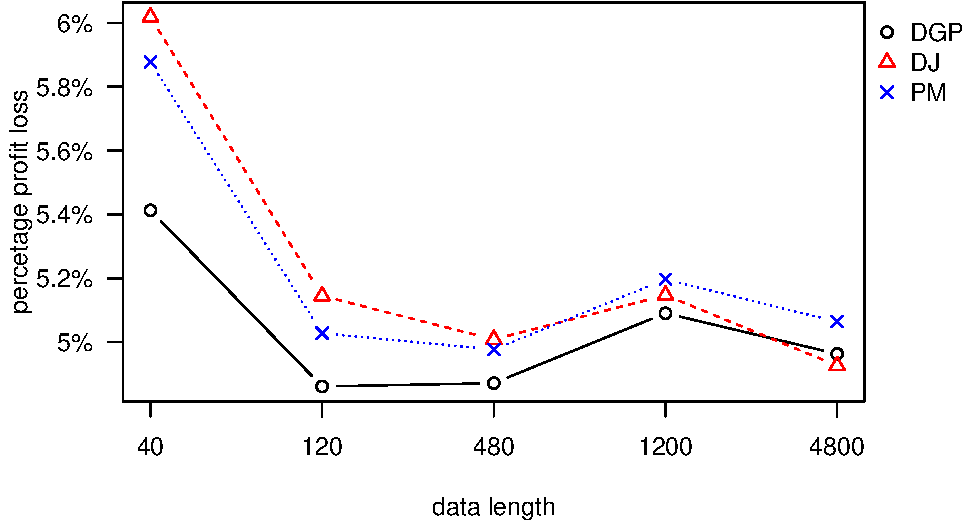
\includegraphics{runif-plot_files/figure-latex/ppl-1.pdf}

\hypertarget{sl-vs-length}{%
\subsection{sl vs length}\label{sl-vs-length}}

\begin{Shaded}
\begin{Highlighting}[]
\NormalTok{x_axis<-}\KeywordTok{c}\NormalTok{(}\DecValTok{40}\NormalTok{,}\DecValTok{120}\NormalTok{,}\DecValTok{480}\NormalTok{,}\DecValTok{1200}\NormalTok{,}\DecValTok{4800}\NormalTok{)}
\NormalTok{y_}\DecValTok{40}\NormalTok{<-}\KeywordTok{c}\NormalTok{(}\KeywordTok{mean}\NormalTok{(}\KeywordTok{sapply}\NormalTok{(re_}\DecValTok{40}\NormalTok{[[}\DecValTok{1}\NormalTok{]], }\StringTok{"[["}\NormalTok{, }\DecValTok{2}\NormalTok{)),}\KeywordTok{mean}\NormalTok{(}\KeywordTok{sapply}\NormalTok{(re_}\DecValTok{40}\NormalTok{[[}\DecValTok{2}\NormalTok{]], }\StringTok{"[["}\NormalTok{, }\DecValTok{2}\NormalTok{)),}
        \KeywordTok{mean}\NormalTok{(}\KeywordTok{sapply}\NormalTok{(re_}\DecValTok{40}\NormalTok{[[}\DecValTok{3}\NormalTok{]], }\StringTok{"[["}\NormalTok{, }\DecValTok{2}\NormalTok{)))}
\NormalTok{y_}\DecValTok{120}\NormalTok{<-}\KeywordTok{c}\NormalTok{(}\KeywordTok{mean}\NormalTok{(}\KeywordTok{sapply}\NormalTok{(re_}\DecValTok{120}\NormalTok{[[}\DecValTok{1}\NormalTok{]], }\StringTok{"[["}\NormalTok{, }\DecValTok{2}\NormalTok{)),}\KeywordTok{mean}\NormalTok{(}\KeywordTok{sapply}\NormalTok{(re_}\DecValTok{120}\NormalTok{[[}\DecValTok{2}\NormalTok{]], }\StringTok{"[["}\NormalTok{, }\DecValTok{2}\NormalTok{)),}
        \KeywordTok{mean}\NormalTok{(}\KeywordTok{sapply}\NormalTok{(re_}\DecValTok{120}\NormalTok{[[}\DecValTok{3}\NormalTok{]], }\StringTok{"[["}\NormalTok{, }\DecValTok{2}\NormalTok{)))}
\NormalTok{y_}\DecValTok{480}\NormalTok{<-}\KeywordTok{c}\NormalTok{(}\KeywordTok{mean}\NormalTok{(}\KeywordTok{sapply}\NormalTok{(re_}\DecValTok{480}\NormalTok{[[}\DecValTok{1}\NormalTok{]], }\StringTok{"[["}\NormalTok{, }\DecValTok{2}\NormalTok{)),}\KeywordTok{mean}\NormalTok{(}\KeywordTok{sapply}\NormalTok{(re_}\DecValTok{480}\NormalTok{[[}\DecValTok{2}\NormalTok{]], }\StringTok{"[["}\NormalTok{, }\DecValTok{2}\NormalTok{)),}
        \KeywordTok{mean}\NormalTok{(}\KeywordTok{sapply}\NormalTok{(re_}\DecValTok{480}\NormalTok{[[}\DecValTok{3}\NormalTok{]], }\StringTok{"[["}\NormalTok{, }\DecValTok{2}\NormalTok{)))}
\NormalTok{y_}\DecValTok{1200}\NormalTok{<-}\KeywordTok{c}\NormalTok{(}\KeywordTok{mean}\NormalTok{(}\KeywordTok{sapply}\NormalTok{(re_}\DecValTok{1200}\NormalTok{[[}\DecValTok{1}\NormalTok{]], }\StringTok{"[["}\NormalTok{, }\DecValTok{2}\NormalTok{)),}\KeywordTok{mean}\NormalTok{(}\KeywordTok{sapply}\NormalTok{(re_}\DecValTok{1200}\NormalTok{[[}\DecValTok{2}\NormalTok{]], }\StringTok{"[["}\NormalTok{, }\DecValTok{2}\NormalTok{)),}
        \KeywordTok{mean}\NormalTok{(}\KeywordTok{sapply}\NormalTok{(re_}\DecValTok{1200}\NormalTok{[[}\DecValTok{3}\NormalTok{]], }\StringTok{"[["}\NormalTok{, }\DecValTok{2}\NormalTok{)))}
\NormalTok{y_}\DecValTok{4800}\NormalTok{<-}\KeywordTok{c}\NormalTok{(}\KeywordTok{mean}\NormalTok{(}\KeywordTok{sapply}\NormalTok{(re_}\DecValTok{4800}\NormalTok{[[}\DecValTok{1}\NormalTok{]], }\StringTok{"[["}\NormalTok{, }\DecValTok{2}\NormalTok{)),}\KeywordTok{mean}\NormalTok{(}\KeywordTok{sapply}\NormalTok{(re_}\DecValTok{4800}\NormalTok{[[}\DecValTok{2}\NormalTok{]], }\StringTok{"[["}\NormalTok{, }\DecValTok{2}\NormalTok{)),}
        \KeywordTok{mean}\NormalTok{(}\KeywordTok{sapply}\NormalTok{(re_}\DecValTok{4800}\NormalTok{[[}\DecValTok{3}\NormalTok{]], }\StringTok{"[["}\NormalTok{, }\DecValTok{2}\NormalTok{)))}
\NormalTok{y_axis<-}\KeywordTok{c}\NormalTok{(y_}\DecValTok{40}\NormalTok{,y_}\DecValTok{120}\NormalTok{,y_}\DecValTok{480}\NormalTok{,y_}\DecValTok{1200}\NormalTok{,y_}\DecValTok{4800}\NormalTok{)}
\NormalTok{mac<-}\KeywordTok{matrix}\NormalTok{(y_axis,}\DataTypeTok{nrow =} \DecValTok{3}\NormalTok{,}\DataTypeTok{ncol =} \DecValTok{5}\NormalTok{)}
\NormalTok{mac<-}\KeywordTok{t}\NormalTok{(mac)}
\KeywordTok{rownames}\NormalTok{(mac)<-}\KeywordTok{c}\NormalTok{(}\StringTok{'40'}\NormalTok{,}\StringTok{'120'}\NormalTok{,}\StringTok{'480'}\NormalTok{,}\StringTok{'1200'}\NormalTok{,}\StringTok{'4800'}\NormalTok{)}
\KeywordTok{colnames}\NormalTok{(mac)<-}\KeywordTok{c}\NormalTok{(}\StringTok{"DGP"}\NormalTok{, }\StringTok{"DJ"}\NormalTok{,}\StringTok{"CF"}\NormalTok{)}
\NormalTok{mac}
\end{Highlighting}
\end{Shaded}

\begin{verbatim}
##          DGP      DJ      CF
## 40   0.18740 0.19940 0.34515
## 120  0.25115 0.22455 0.30870
## 480  0.28420 0.23565 0.30015
## 1200 0.29620 0.24150 0.30230
## 4800 0.29925 0.23880 0.30470
\end{verbatim}

\begin{Shaded}
\begin{Highlighting}[]
\NormalTok{v_}\DecValTok{40}\NormalTok{<-}\KeywordTok{c}\NormalTok{(}\KeywordTok{sd}\NormalTok{(}\KeywordTok{sapply}\NormalTok{(re_}\DecValTok{40}\NormalTok{[[}\DecValTok{1}\NormalTok{]], }\StringTok{"[["}\NormalTok{, }\DecValTok{2}\NormalTok{)),}\KeywordTok{sd}\NormalTok{(}\KeywordTok{sapply}\NormalTok{(re_}\DecValTok{40}\NormalTok{[[}\DecValTok{2}\NormalTok{]], }\StringTok{"[["}\NormalTok{, }\DecValTok{2}\NormalTok{)),}
        \KeywordTok{sd}\NormalTok{(}\KeywordTok{sapply}\NormalTok{(re_}\DecValTok{40}\NormalTok{[[}\DecValTok{3}\NormalTok{]], }\StringTok{"[["}\NormalTok{, }\DecValTok{2}\NormalTok{)))}
\NormalTok{v_}\DecValTok{120}\NormalTok{<-}\KeywordTok{c}\NormalTok{(}\KeywordTok{sd}\NormalTok{(}\KeywordTok{sapply}\NormalTok{(re_}\DecValTok{120}\NormalTok{[[}\DecValTok{1}\NormalTok{]], }\StringTok{"[["}\NormalTok{, }\DecValTok{2}\NormalTok{)),}\KeywordTok{sd}\NormalTok{(}\KeywordTok{sapply}\NormalTok{(re_}\DecValTok{120}\NormalTok{[[}\DecValTok{2}\NormalTok{]], }\StringTok{"[["}\NormalTok{, }\DecValTok{2}\NormalTok{)),}
        \KeywordTok{sd}\NormalTok{(}\KeywordTok{sapply}\NormalTok{(re_}\DecValTok{120}\NormalTok{[[}\DecValTok{3}\NormalTok{]], }\StringTok{"[["}\NormalTok{, }\DecValTok{2}\NormalTok{)))}
\NormalTok{v_}\DecValTok{480}\NormalTok{<-}\KeywordTok{c}\NormalTok{(}\KeywordTok{sd}\NormalTok{(}\KeywordTok{sapply}\NormalTok{(re_}\DecValTok{480}\NormalTok{[[}\DecValTok{1}\NormalTok{]], }\StringTok{"[["}\NormalTok{, }\DecValTok{2}\NormalTok{)),}\KeywordTok{sd}\NormalTok{(}\KeywordTok{sapply}\NormalTok{(re_}\DecValTok{480}\NormalTok{[[}\DecValTok{2}\NormalTok{]], }\StringTok{"[["}\NormalTok{, }\DecValTok{2}\NormalTok{)),}
        \KeywordTok{sd}\NormalTok{(}\KeywordTok{sapply}\NormalTok{(re_}\DecValTok{480}\NormalTok{[[}\DecValTok{3}\NormalTok{]], }\StringTok{"[["}\NormalTok{, }\DecValTok{2}\NormalTok{)))}
\NormalTok{v_}\DecValTok{1200}\NormalTok{<-}\KeywordTok{c}\NormalTok{(}\KeywordTok{sd}\NormalTok{(}\KeywordTok{sapply}\NormalTok{(re_}\DecValTok{1200}\NormalTok{[[}\DecValTok{1}\NormalTok{]], }\StringTok{"[["}\NormalTok{, }\DecValTok{2}\NormalTok{)),}\KeywordTok{sd}\NormalTok{(}\KeywordTok{sapply}\NormalTok{(re_}\DecValTok{1200}\NormalTok{[[}\DecValTok{2}\NormalTok{]], }\StringTok{"[["}\NormalTok{, }\DecValTok{2}\NormalTok{)),}
        \KeywordTok{sd}\NormalTok{(}\KeywordTok{sapply}\NormalTok{(re_}\DecValTok{1200}\NormalTok{[[}\DecValTok{3}\NormalTok{]], }\StringTok{"[["}\NormalTok{, }\DecValTok{2}\NormalTok{)))}
\NormalTok{v_}\DecValTok{4800}\NormalTok{<-}\KeywordTok{c}\NormalTok{(}\KeywordTok{sd}\NormalTok{(}\KeywordTok{sapply}\NormalTok{(re_}\DecValTok{4800}\NormalTok{[[}\DecValTok{1}\NormalTok{]], }\StringTok{"[["}\NormalTok{, }\DecValTok{2}\NormalTok{)),}\KeywordTok{sd}\NormalTok{(}\KeywordTok{sapply}\NormalTok{(re_}\DecValTok{4800}\NormalTok{[[}\DecValTok{2}\NormalTok{]], }\StringTok{"[["}\NormalTok{, }\DecValTok{2}\NormalTok{)),}
        \KeywordTok{sd}\NormalTok{(}\KeywordTok{sapply}\NormalTok{(re_}\DecValTok{4800}\NormalTok{[[}\DecValTok{3}\NormalTok{]], }\StringTok{"[["}\NormalTok{, }\DecValTok{2}\NormalTok{)))}
\NormalTok{v_axis<-}\KeywordTok{c}\NormalTok{(v_}\DecValTok{40}\NormalTok{,v_}\DecValTok{120}\NormalTok{,v_}\DecValTok{480}\NormalTok{,v_}\DecValTok{1200}\NormalTok{,v_}\DecValTok{4800}\NormalTok{)}
\NormalTok{var<-}\KeywordTok{matrix}\NormalTok{(v_axis,}\DataTypeTok{nrow =} \DecValTok{3}\NormalTok{,}\DataTypeTok{ncol =} \DecValTok{5}\NormalTok{)}
\NormalTok{var<-}\KeywordTok{t}\NormalTok{(var)}
\KeywordTok{rownames}\NormalTok{(var)<-}\KeywordTok{c}\NormalTok{(}\StringTok{'40'}\NormalTok{,}\StringTok{'120'}\NormalTok{,}\StringTok{'480'}\NormalTok{,}\StringTok{'1200'}\NormalTok{,}\StringTok{'4800'}\NormalTok{)}
\KeywordTok{colnames}\NormalTok{(var)<-}\KeywordTok{c}\NormalTok{(}\StringTok{"DGP"}\NormalTok{, }\StringTok{"DJ"}\NormalTok{,}\StringTok{"CF"}\NormalTok{)}
\NormalTok{var}
\end{Highlighting}
\end{Shaded}

\begin{verbatim}
##            DGP        DJ        CF
## 40   0.3902420 0.3995593 0.4754290
## 120  0.4336855 0.4172961 0.4619686
## 480  0.4510438 0.4244150 0.4583345
## 1200 0.4565917 0.4280034 0.4592660
## 4800 0.4579410 0.4263609 0.4602918
\end{verbatim}

\begin{Shaded}
\begin{Highlighting}[]
\KeywordTok{par}\NormalTok{(}\DataTypeTok{mar=}\KeywordTok{c}\NormalTok{(}\KeywordTok{par}\NormalTok{(}\StringTok{'mar'}\NormalTok{)[}\DecValTok{1}\OperatorTok{:}\DecValTok{3}\NormalTok{], }\DecValTok{0}\NormalTok{)) }
\KeywordTok{plot.new}\NormalTok{()}
\NormalTok{l <-}\StringTok{ }\KeywordTok{legend}\NormalTok{(}\DecValTok{0}\NormalTok{, }\DecValTok{0}\NormalTok{, }\DataTypeTok{bty=}\StringTok{'n'}\NormalTok{,}\KeywordTok{c}\NormalTok{(}\StringTok{"DGP"}\NormalTok{, }\StringTok{"DJ"}\NormalTok{,}\StringTok{"PM"}\NormalTok{),}\DataTypeTok{plot=}\OtherTok{FALSE}\NormalTok{, }\DataTypeTok{pch=}\DecValTok{1}\OperatorTok{:}\DecValTok{3}\NormalTok{,}\DataTypeTok{col=}\DecValTok{1}\OperatorTok{:}\DecValTok{3}\NormalTok{)}
\NormalTok{w <-}\StringTok{ }\KeywordTok{grconvertX}\NormalTok{(l}\OperatorTok{$}\NormalTok{rect}\OperatorTok{$}\NormalTok{w, }\DataTypeTok{to=}\StringTok{'ndc'}\NormalTok{) }\OperatorTok{-}\StringTok{ }\KeywordTok{grconvertX}\NormalTok{(}\DecValTok{0}\NormalTok{, }\DataTypeTok{to=}\StringTok{'ndc'}\NormalTok{)}
\KeywordTok{par}\NormalTok{(}\DataTypeTok{omd=}\KeywordTok{c}\NormalTok{(}\DecValTok{0}\NormalTok{, }\DecValTok{1}\OperatorTok{-}\NormalTok{w, }\DecValTok{0}\NormalTok{, }\DecValTok{1}\NormalTok{))}
\KeywordTok{matplot}\NormalTok{(mac, }\DataTypeTok{type =} \KeywordTok{c}\NormalTok{(}\StringTok{"b"}\NormalTok{),}\DataTypeTok{pch=}\DecValTok{1}\OperatorTok{:}\DecValTok{3}\NormalTok{,}\DataTypeTok{col =} \DecValTok{1}\OperatorTok{:}\DecValTok{3}\NormalTok{,}\DataTypeTok{xaxt =} \StringTok{"n"}
\NormalTok{        ,}\DataTypeTok{xlab =} \StringTok{'data length'}\NormalTok{,}\DataTypeTok{ylab =} \StringTok{'service level'}\NormalTok{) }
\KeywordTok{axis}\NormalTok{(}\DecValTok{1}\NormalTok{, }\DataTypeTok{at=}\DecValTok{1}\OperatorTok{:}\DecValTok{5}\NormalTok{, }\DataTypeTok{labels=}\NormalTok{x_axis)}
\KeywordTok{legend}\NormalTok{(}\KeywordTok{par}\NormalTok{(}\StringTok{'usr'}\NormalTok{)[}\DecValTok{2}\NormalTok{], }\KeywordTok{par}\NormalTok{(}\StringTok{'usr'}\NormalTok{)[}\DecValTok{4}\NormalTok{], }\DataTypeTok{bty=}\StringTok{'n'}\NormalTok{, }\DataTypeTok{xpd=}\OtherTok{NA}
\NormalTok{       ,}\KeywordTok{c}\NormalTok{(}\StringTok{"DGP"}\NormalTok{, }\StringTok{"DJ"}\NormalTok{,}\StringTok{"PM"}\NormalTok{), }\DataTypeTok{pch=}\DecValTok{1}\OperatorTok{:}\DecValTok{3}\NormalTok{,}\DataTypeTok{col=}\DecValTok{1}\OperatorTok{:}\DecValTok{3}\NormalTok{)}
\end{Highlighting}
\end{Shaded}

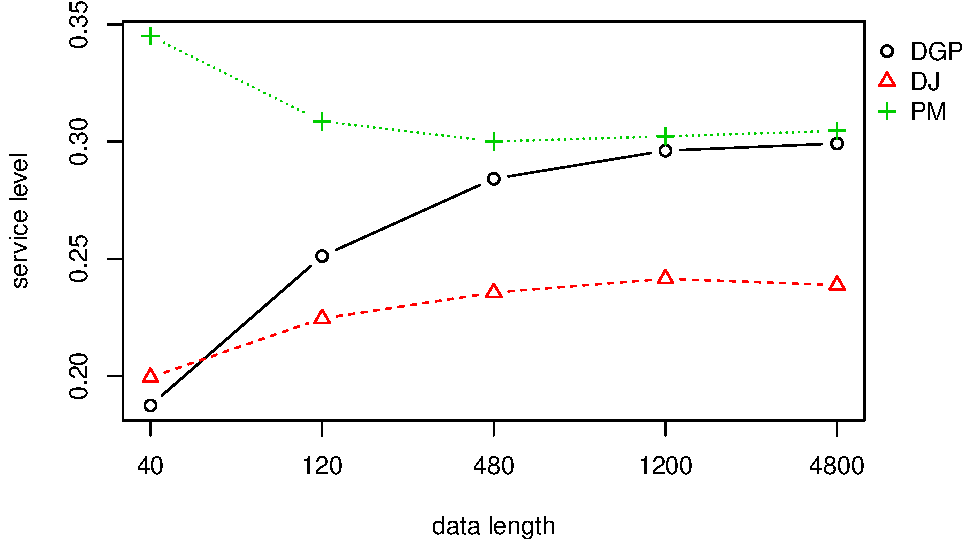
\includegraphics{runif-plot_files/figure-latex/sl-1.pdf}

\end{document}
